\newpage
\phantomsection
\addcontentsline{toc}{subsection}{\textsl{Diwar Les Coet}}
\thispagestyle{empty}

\section*{\textsl{Diwar Les Coet}}
\label{dlcscore}

\begin{center} 
\textbf{Composition Ouverte Opus 1}

{\scriptsize  \texttt{Copyleft \textcopyleft \, 2014/2017 Yann Ics - All Wrongs Reserved.}}
 \end{center} 
 \begin{figure}[H]
%\begin{center}
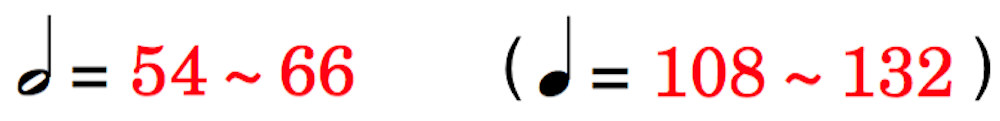
\includegraphics[scale=0.1]{img/dlct}
%\end{center}
\end{figure}
 
 Le tempo est purement indicatif et peut varier significativement et de manière dynamique, pourvu qu'il soit partager par tous les acteurs de la performance, qu'il soit synchronisé ou non.

\subsection*{Choral}

Initialement écrit pour 3 voix d'hommes, le choral peut être interprété librement par toutes les voix et adapté par octaviation. Les notes longues peuvent être monnayées ou vocalisées à loisirs selon le (con)texte. 

 \begin{figure}[H]
\begin{center}
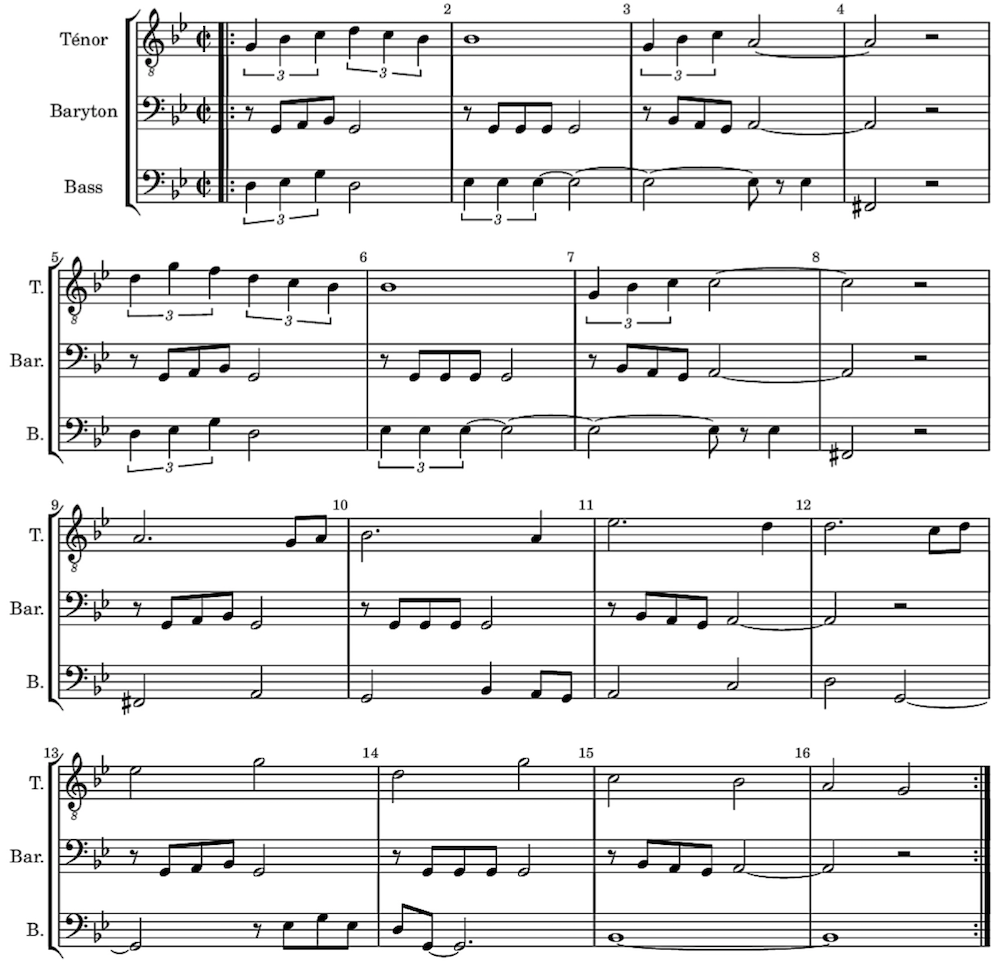
\includegraphics[scale=0.68]{img/dlc1}
\end{center}
\end{figure}

Pour certain passage, une version murmurée ou bouche fermée entre bien entendu dans le domaine du possible.

%Le choral peut faire office de choeur et être accompagné d'une (ou de) mélodie(s) soliste(s).

Voici les combinaisons possibles (1 =  ténor, 2 = baryton et 3 =  bass): 

1-- 2 -- 3 -- 12 -- 13 -- 23 -- 123

\subsection*{Variations pour Guitares}
Les grilles d'accords des guitares sont indicatives et peuvent par conséquent être adaptées librement au jeu du guitariste ou modifiées selon l'interprétation souhaitée. La première grille étant la référence harmonique simplifiée.

 \begin{figure}[H]
\begin{center}
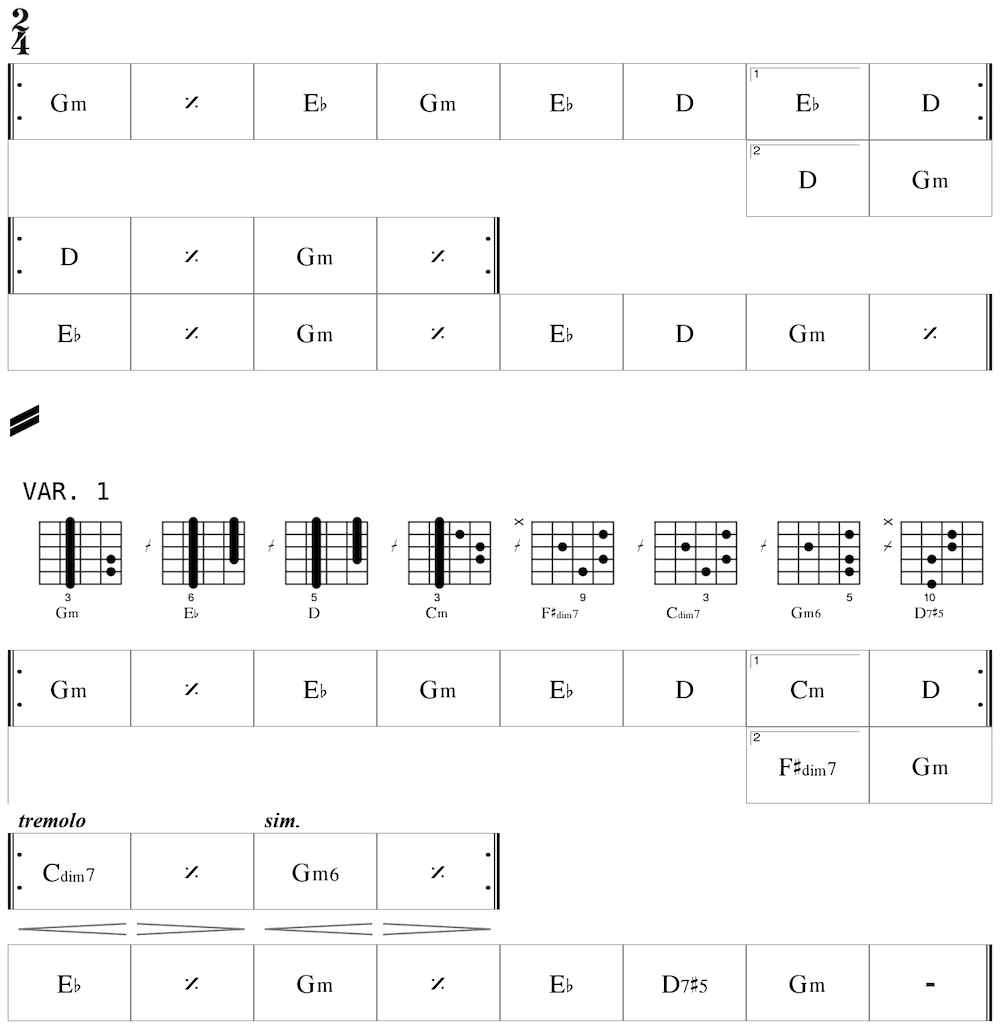
\includegraphics[scale=0.33]{img/dlc2}
\end{center}
\end{figure}
Le cas échéant, les grilles harmoniques peuvent être réalisées par n'importe quel instrument ou formation.
 
 \begin{figure}[H]
\begin{center}
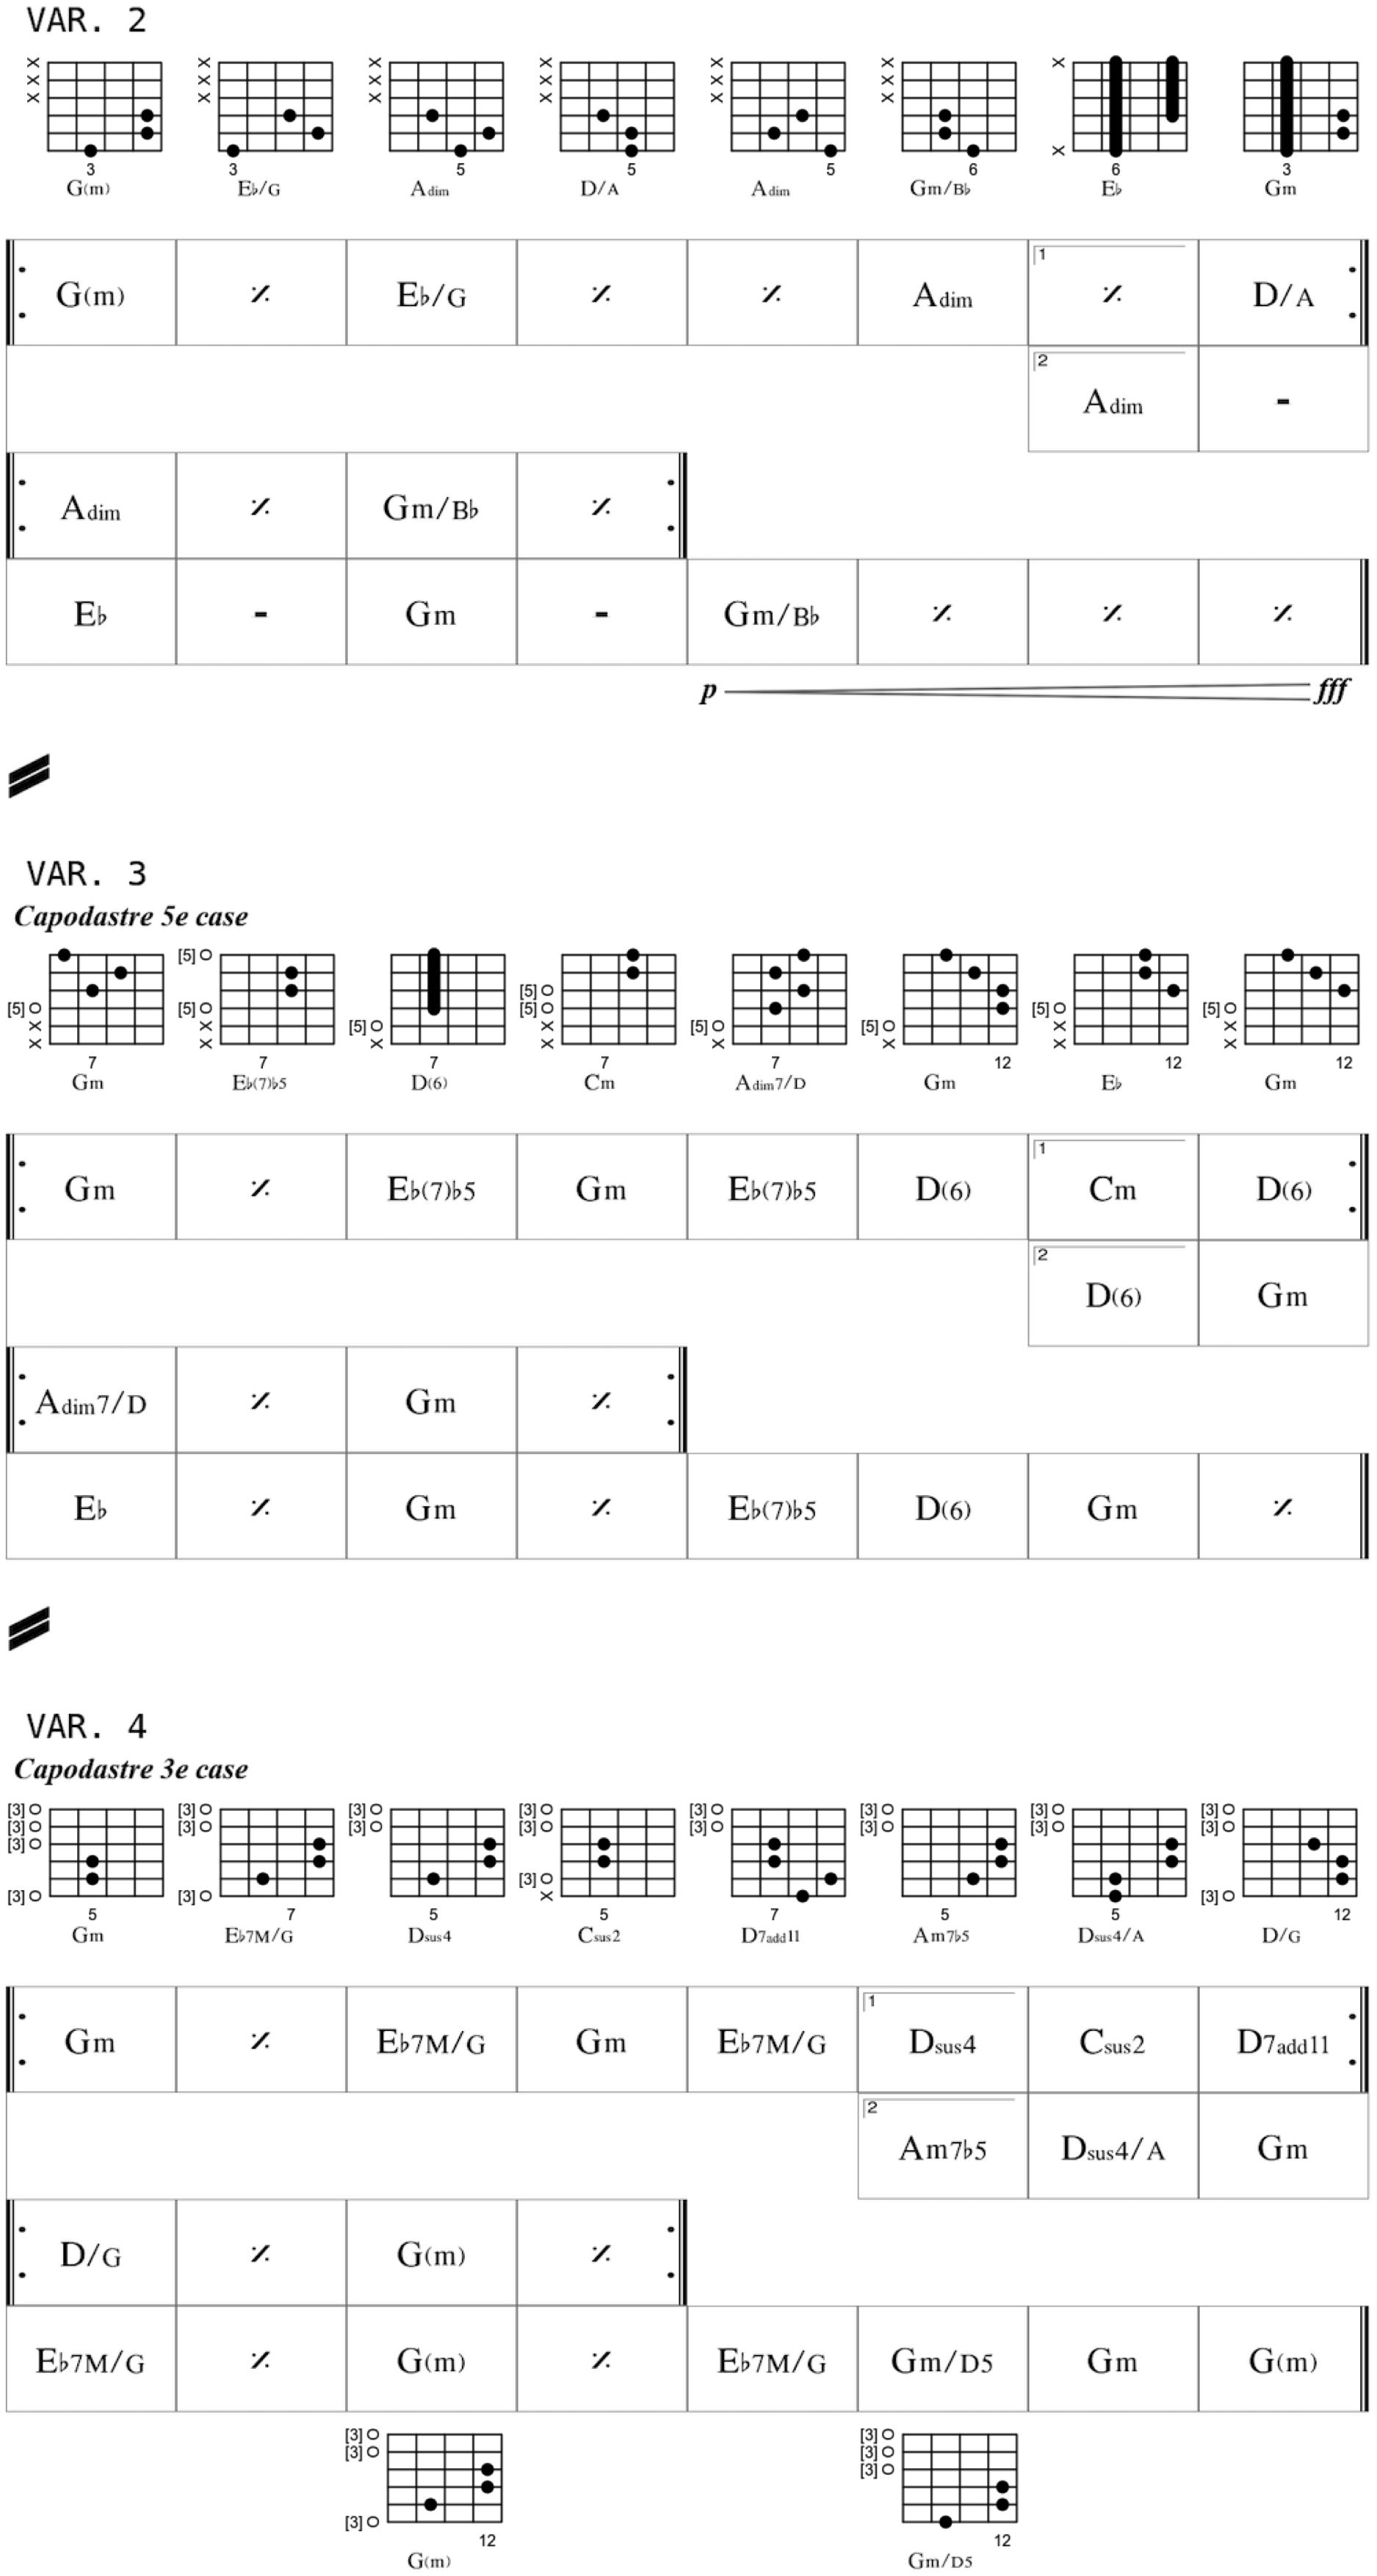
\includegraphics[scale=0.33]{img/dlc3}
\end{center}
\end{figure}

 \begin{figure}[H]
\begin{center}
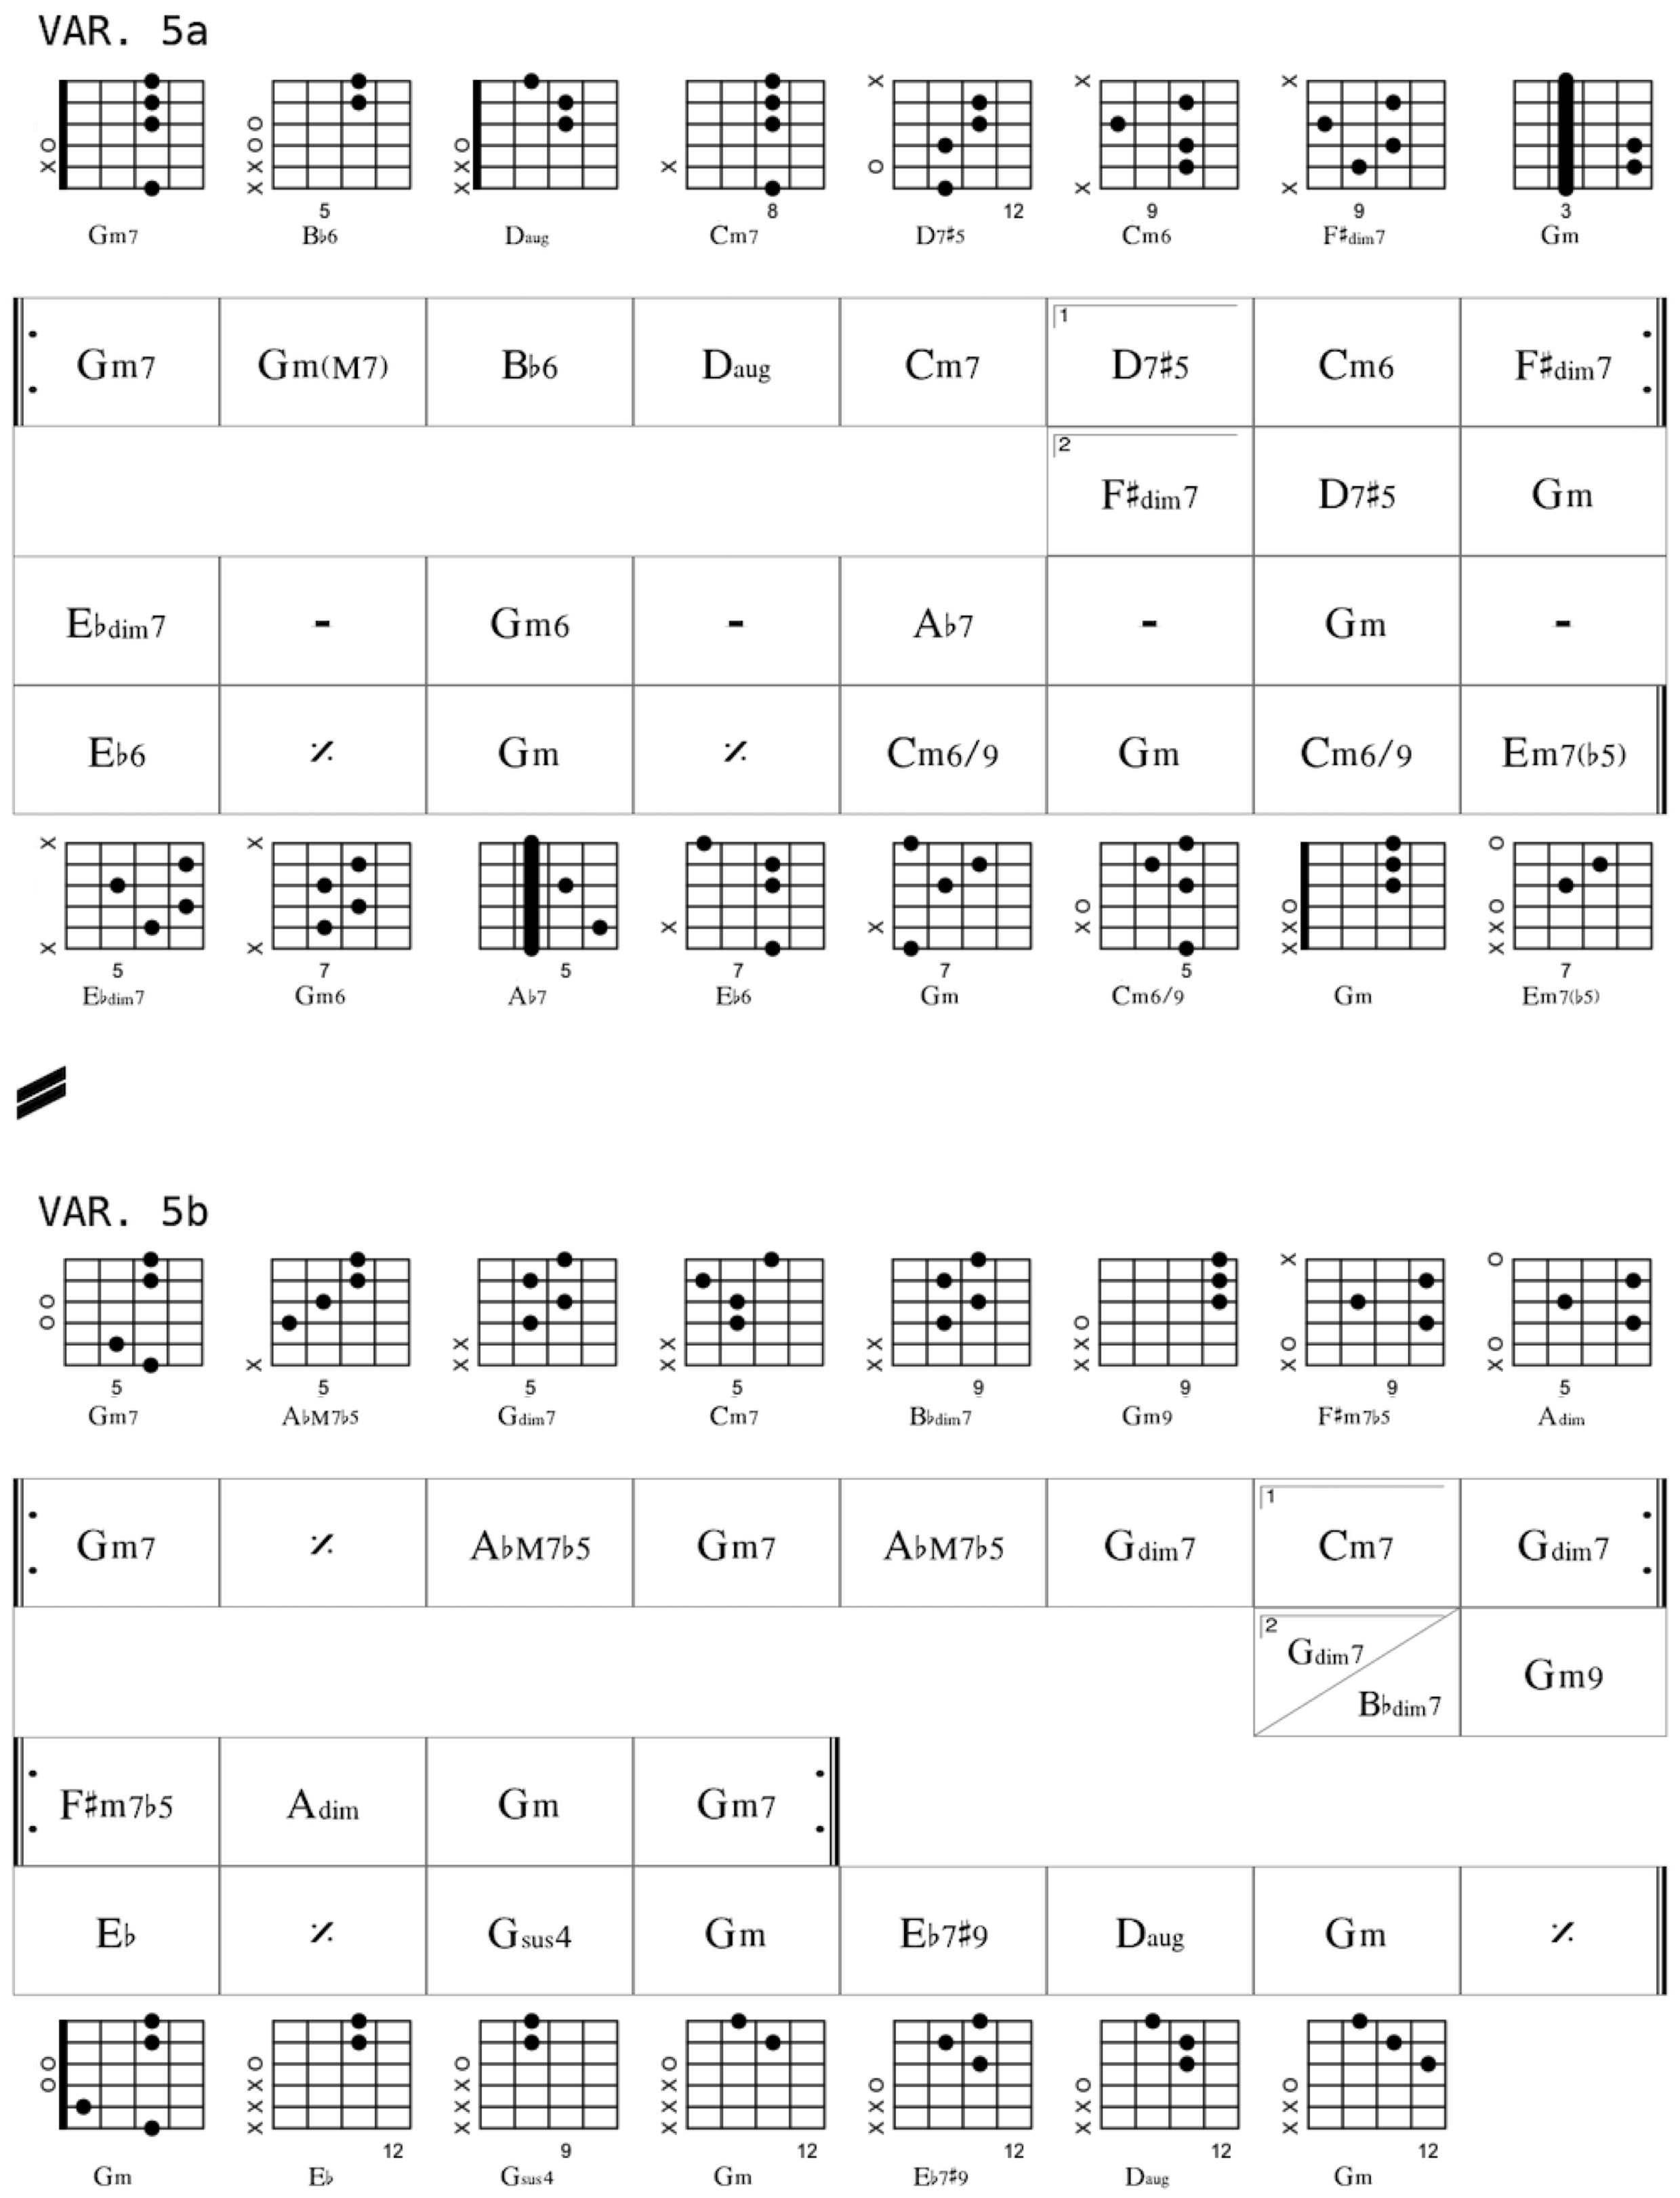
\includegraphics[scale=0.33]{img/dlc4}
\end{center}
\end{figure}

Voici les combinaisons possibles selon les grilles proposées (1 = variation 1, 2 = variation 2, 3 = variation 3 et 4 = variation 4, 5 = variation 5a, et 6 = variation 5b) pour 4 guitaristes: 

1 -- 2 -- 3 -- 4 -- 5 -- 6 -- 12 -- 13 -- 14 -- 15 -- 16 --  23 -- 24 -- 25 --26 -- 34 -- 35 -- 36 -- 45 -- 46 -- 56 -- 123 -- 124 -- 134 -- 135 -- 136 -- 234 -- 235 -- 236 -- 345 -- 346 -- 456 -- 1234 -- 1235 -- 1236 --2345 -- 2346 -- 3456 %-- 12345 -- 12346 -- 23456 -- 123456
 
\bigskip

\subsection*{Thème Rythmique -- djembé/dum-dum}

Les percussions sont définies ici -- par défaut -- par le couple djembé/dumdum, mais peuvent bien entendu être adaptées selon un \textit{instrumentarium} libre et selon des motifs rythmiques autres, mais apparentés.

 %La séquence présentée ici est un exemple.
 
 \begin{figure}[H]
\begin{center}
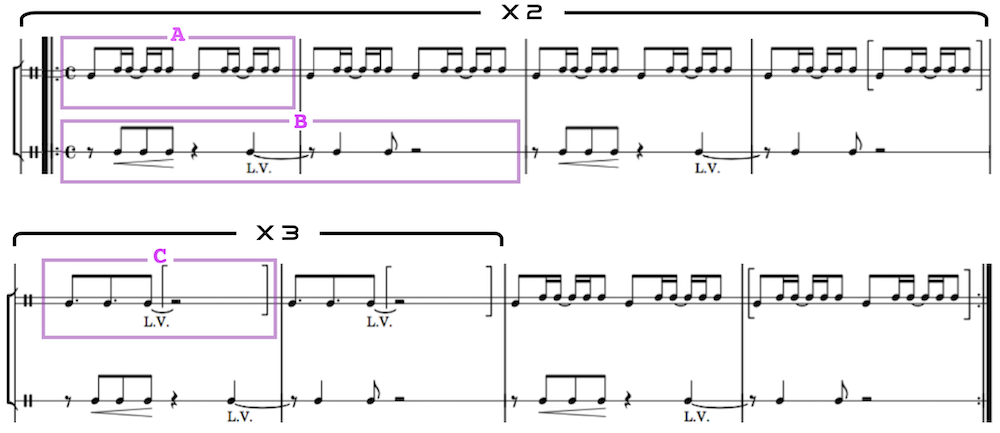
\includegraphics[scale=0.68]{img/dlc5}
\end{center}
\end{figure}

À l’instar des briques d’une construction, chaque motif rythmique --  ici encadré et dénommé A, B et C -- est agencé afin d’entrer dans l’élaboration d’une séquence entière, soit 16 mesures.

Les parties entre crochets doivent être interprétées en termes d'articulation et/ou de cadence selon le contexte.
